%
% 53-homologie.tex -- Homologie von Ketten
%
% (c) 2026 Prof Dr Andreas Müller
%
\subsection{Homologie von Ketten
\label{buch:integration:homologie:subsection:homologie}}
Die Homotpieeigenschaft des Wegintegrals hat gezeigt, dass sich der
Wert eines Wegintegrals einer holomorphen Funktion nicht ändert, wenn
man den Weg stetig deformiert.
Dies wurde zum Beispiel in
Abbildung~\ref{buch:integration:homologie:fig:residuum}
verwendet, um zu zeigen, dass der Weg $\gamma$ und der kleine Kreis
um den Punkt $z_0$ zu den gleichen Werten der Wegintegrale führen.
Diese Äquivalenz von Ketten, die zu gleichen Wegintegralen führen,
verdient einen eigenen Namen.

\begin{definition}[homolog]
Die geschlossene Ketten $c_1$ und $c_2$ heissen \emph{homolog} in $U$,
in Zeichen $c_1\sim c_2$ oder $c_1\sim_{U}c_2$, wenn
\index{homolog}%
für jeden Punkt $a\in \mathbb{C}\setminus U$ ausserhalb von $U$
die Umlaufzahlen
\[
\operatorname{ind}_{c_1}(a)
=
\operatorname{ind}_{c_2}(a)
\]
von $c_1$ und $c_2$ um $a$ gleich sind.
\end{definition}

Die Kette $\gamma_++\gamma_-$ in
Abbildung~\ref{buch:integration:homologie:fig:paar} ist zu $\gamma$ homolog,
da beide Ketten jedes der Löcher $F_1$ und $F_2$ genau einmal umrunden.
Für homologe Ketten ist nicht nur die Umlaufzahl gleich, sondern
jedes Integral einer holomorphen Funktion über die Ketten.

\begin{satz}
\label{buch:integration:homologie:satz:cauchyketten}
Sei $U$ ein Gebiet in $\mathbb{C}$ und
$c$ eine Kette, die homolog zu $0$ ist.
Dann ist
\[
\int_c f(z)\,dz = 0
\]
für jede in $U$ holomorphe Funktion.
\end{satz}

Aus diesem Satz folgt sofort das folgende Korollar.
Es zeigt, dass es bei Kettenintegralen von holomorphen Funktionen
nur auf die Homologieklasse der Kette ankommt, über die integriert
wird.
Sind Ketten homolog, ergibt sich auch der gleiche Wert des Integrals.

\begin{korollar}
Sind die Ketten $c_1$ und $c_2$ homolog, dann ist
\[
\int_{c_1} f(z)\,dz
=
\int_{c_2} f(z)\,dz.
\]
\end{korollar}

\begin{proof}
Die Kette $c=c_1-c_2$ ist homolog zu 0 und daher
\[
0
=
\int_c f(z)\,dz
=
\int_{c_1}f(z)\,dz - \int_{c_2}f(z)\,dz
\qquad\Rightarrow\qquad
\int_{c_1}f(z)\,dz = \int_{c_2}f(z)\,dz.
\qedhere
\]
\end{proof}

Der Satz~\ref{buch:integration:homologie:satz:cauchyketten}
macht keine Voraussetzung weiteren Voraussetzungen an die Funktion
als dass sie in $U$ holomorph sein muss.
Die Funktionen $z\mapsto 1/(z-z_0)$ mit $z_0\in\mathbb{C}\setminus U$
sind alle holomorph in $U$.
Die Integrale über die Kette ergeben die Umlaufzahlen.
Da die Ketten 0-homolog sind, müssen alle diese Umlaufzahlen 0
ergeben.

Für beliebige Funktionen $f(z)$ können wir in der Umgebung eines
Punktes immer eine lokale Stammfunktion finden, die ausserdem
unabhängig ist vom Weg.
Zum Beispiel wissen wir schon, dass Wegintegrale über den Rand
von Rechtecke immer verschwinden, wenn $f(z)$ holomorph ist im
ganzen Rechteck.
Auch wissen wir dies bereits für geschlossene und zusammenziehbare
Wege.
Die Hauptaufgabe des Beweises ist also, diese Erkenntnisse auf 
Ketten zu verallgemeinern, die weit auseinanderliegende Komponenten
haben können.

Um den Satz zu beweisen, verfolgen wir die folgende Strategie.
\begin{enumerate}
\item
Zunächst approximieren wir die Kette durch eine Kette, deren
Wege alle aus achsenparallelen Segmenten bestehen.
Die Kettenintegrale ändern sich dadurch nicht.
\item
Wir zerlegen den achsenparallelen Weg in eine Summe von Rändern
von Rechtecken, die vollständig in $U$ enthalten sind.
\item 
Wir berechnen das Integral über die Kette als Summe über die Integrale
über die Ränder der Rechtecke.
\end{enumerate}

%
% fig-treppe.tex
%
% (c) 2026 Prof Dr Andreas Müller
%
\begin{figure}
\centering
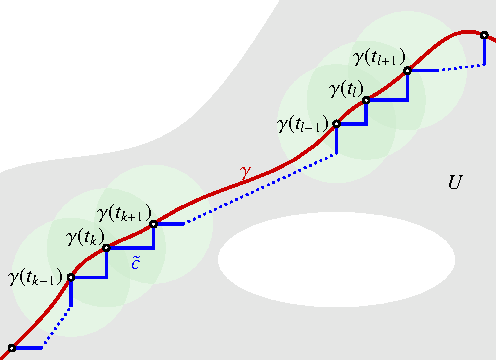
\includegraphics{chapters/030-integration/images/treppe.pdf}
\caption{Approximation eines Weges $\gamma$ in einer Kette durch eine Kette
von achsenparallelen Segmenten $\tilde{c}$.
\label{buch:integration:fig:treppe}}
\end{figure}
%

%
% fig-gitterapprox.tex -- Beweis des Homologie-Satzes
%
% (c) 2026 Prof Dr Andreas Müller
%
\begin{figure}
\centering
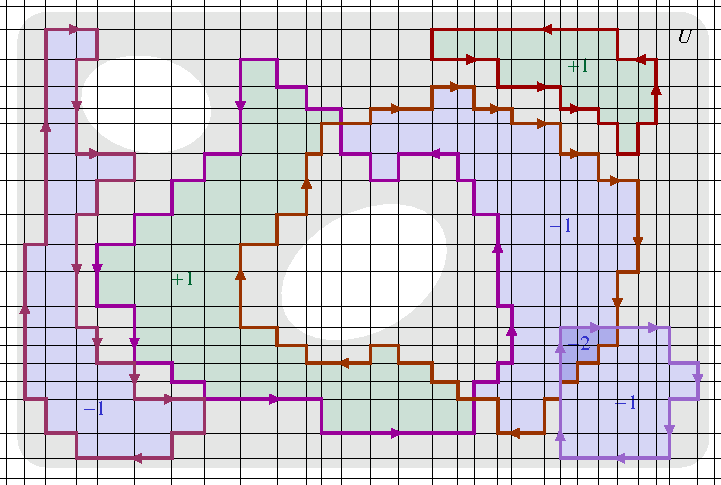
\includegraphics{chapters/030-integration/images/gitterapprox.pdf}
\caption{Eine nullhomologe Kette lässt sich durch eine nullhomologen Kette
$c$ mit achsparallelen Segmenten approximieren, ohne dass sich
Integrale ändern.
Die Segmente definieren eine Unterteilung der Ebene in Rechtecke.
Jedem Rechteck $R_i$ wird die Umlaufzahl $m_i=\operatorname{ind}_{c}(a_i)$
eines Punktes $a_i\in R_i$ zugeordnet.
Die farbigen Rechtecke haben $m_i\ne 0$.
Die Kette ist $c=\sum_i m_i\partial R_i$.
\label{buch:integration:fig:gitterapprox}}
\end{figure}
%

\begin{proof}[Beweis von Satz~\ref{buch:integration:homologie:satz:cauchyketten}]
\begin{enumerate}
\item
Approximation des Weges $\gamma$.

Die Kette $c$ besteht aus einzelnen differenzierbaren Wegen $\gamma$.
Mit jedem Punkt einer Kurve ist auch eine genügend kleine Kreisscheibe
um den Punkt in $U$ enthalten (Abbildung~\ref{buch:integration:fig:treppe}).
Da die Kurve kompakt ist, kann man sie mit endlich vielen solchen Kreisen
abdecken.
In jeder Kreisscheibe kann man auf dem Weg Punkte auswählen, so dass 
zu jeweils zwei aufeinanderfolgenden Punkten auf dem Weg auch das von
den Punkte aufgespannte Rechteck in $U$ ist.
Der Weg kann also durch Teile des Randes dieser Rechtecke ersetzt werden.
Die Umlaufzahlen und Integrale ändern sich dabei nicht, da die 
Rechtecke so klein sind, dass das die Funktionen eine Stammfunktion haben.
Wir ersetzen die Ketten durch eine Kette bestehend aus diesen Randsegmenten.

\item
Aufteilung der Ebene in Rechtecke.

Wir zerlegen die komplexe Ebene durch achsparallele Geraden durch
alle Eckpunkte, die bei der Unterteilung der Kette gefunden wurden
(Abbildung~\ref{buch:integration:fig:gitterapprox}).
Dadurch werden einige der achsparallelen Segmente weiter unterteilt.
Wir bezeichnen die Rechtecke mit $R_i$ und ersetzen die Kette
durch Randsegmente dieser Rechecke.

\item
Selektion der Rechtecke.

In jedem Rechteck wählen wir einen Punkt $\alpha_i\in R_i$ und berechnen
die Umlaufzahl $m_i=\operatorname{ind}_\gamma(\alpha_i)$.
Die Umlaufzahl ist im Inneren jedes Rechtecks konstant.
Wenn $m_i\ne 0$ ist, dann muss $R_i\in U$ sein, denn Punkte ausserhalb
von $U$ würden eine Umlaufzahl $0$ geben, weil $c$ nullhomolog ist.

\item $\displaystyle c=\sum_i m_i\partial R_i$.

%
% fig-nachbar.tex
%
% (c) 2026 Prof Dr Andreas Müller
%
\begin{figure}
\centering
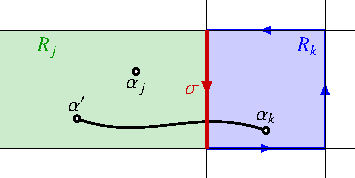
\includegraphics{chapters/030-integration/images/nachbar.pdf}
\caption{Fehlerhafte Kante $\sigma$ des Rechtecks $R_k$ mit Nachbarrechteck $R_j$
für den letzten Schritt des Beweises von Satz
\ref{buch:integration:homologie:satz:cauchyketten}.
\label{buch:integration:fig:nachbar}}
\end{figure}


Angenommen, eine Kante $\sigma$ eines der Rechtecke ist nicht mit der korrekten
Anzahl in $c$ (Abbildung~\ref{buch:integration:fig:nachbar}).
Sei $R_k$ dieses Rechteck.
Dann gibt es eine ganze Zahl $m$ derart, dass
\[
C
=
c-\sum_i m_i\partial R_i - m\partial R_k
\]
die Kante nicht mehr enthält.
Sei $R_j$ das ebenfalls an die Kante $\sigma$ angrenzende Rechteck und
$\alpha'$ ein Punkt in diesem Rechteck.
Da $\sigma$ in $C$ nicht mehr vorkommt, kann man einen Punkt stetig von $\alpha_k$
nach $\alpha'$ verschieben, ohne $C$ zu kreuzen.
Die Umlaufzahl von $C$ kann sich dabei nicht ändern, also muss $C$ gleiche
Umlaufzahlen um  $\alpha_k$ und $\alpha'$ haben.
Andererseits ist die Umlaufzahl linear, d.~h. 
\begin{align*}
\operatorname{ind}_C(\alpha_k)
&=
\operatorname{ind}_{c-\sum_i m_i\partial R_i - m\partial R_k}(\alpha_k)
\\
&=
\operatorname{ind}_c(\alpha_k)
-
\sum_i m_i\operatorname{ind}_{\partial R_i}(\alpha_k)
-
m\operatorname{ind}_{\partial R_k}(\alpha_k)
\\
&=
\operatorname{ind}_c(\alpha_k)
-
\sum_i m_i\delta_{ik}
-
m.
\intertext{Der erste Term ist nach der Definition der Zahlen $m_i$}
&= m_k - m_k - m.
\end{align*}
Andererseits ist $\operatorname{ind}_C(\alpha')$ zu bestimmen.
Falls $\alpha'$ in einem unendlichen Rechteck liegt, ist 
$\operatorname{ind}_C(\alpha')=0$.
Falls $R_j$ ein endliches Rechteck ist, dann ist
$\operatorname{ind}_{c}(\alpha')=\operatorname{ind}_c(\alpha_j)$
und es folgt
\begin{align*}
\operatorname{ind}_C(\alpha')
&=
\operatorname{ind}_{c-\sum_i m_i\partial R_i - m\partial R_k}(\alpha_j)
\\
&=
\operatorname{ind}_{c}(\alpha_j)
-
\sum_i m_i\operatorname{ind}_{\partial R_i}(\alpha_j)
-
m\operatorname{ind}_{\partial R_k}(\alpha_j)
\\
&=
m_j - \sum_i m_i\delta_{ij}
=
m_j-m_j 0 0.
\end{align*}
In beiden Fällen ist $\operatorname{ind}_C(\alpha')=0$ und es folgt,
dass $m=0$, d.~h.~$\sigma$ kam in der Kette gar nicht mit der falschen
Anzahl vor.
\qedhere
\end{enumerate}
\end{proof}

Wir betrachten jetzt einen später besonders nützlichen Spezialfall.
%
% fig-merohomolog.tex
%
% (c) 2026 Prof Dr Andreas Müller
%
\begin{figure}
\centering
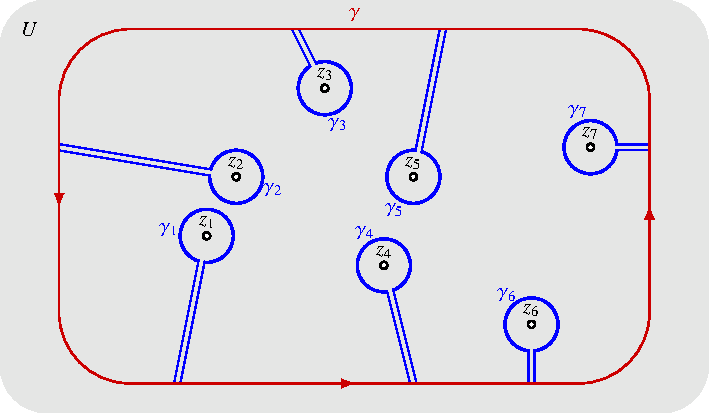
\includegraphics{chapters/030-integration/images/merohomolog.pdf}
\caption{
\label{buch:integration:homologie:fig:merohomolog}}
\end{figure}
%
In Abbildung~\ref{buch:integration:homologie:fig:merohomolog}
ist ein Gebiet $U$ mit einer einfach geschlossenen Kurve
$\gamma$ dargestellt.
Das Komplement von $U$ im Inneren der Kurve $\gamma$ besteht
aus den isolierten Punkten $z_k$.
Jeder dieser Punkte kann so mit der Kurve $\gamma$ verbunden werden,
dass sich die Verbindungen nicht schneiden.
Ausserdem wird jeder von diesen Punkten von einem kleinen Kreis $\gamma_k$
im Gegenuhrzeigersinn umlaufen.
Aus $\gamma$, den im Uhrzeigersinn durchlaufenen Kreisen $-\gamma_k$
und den Verbindungen zu $\gamma$ lässt sich ein neuer Weg zusammensetzen,
der sich in $U$ zusammenziehen lässt.
Das Wegintegral über den gesamten Weg verschwindet daher.
Die Verbindungswege zur Kurve $\gamma$ werden dabei zweimal in
entgegengesetzter Richtung durchlaufen und tragen somit nicht zum
Wegintegral bei.
Das Wegintegral einer in $U$ holomorphen Funktion über $\gamma$
ist daher gleich der Summe der Wegintegrale der Funktion
über die Kreise $\gamma_k$.

\begin{satz}
\label{buch:integration:homologie:satz:pfadpunkte}
Ist $\gamma$ eine einfach geschlossene Kurve in $U$ und besteht das Komplement
von $U$ im Inneren von $\gamma$ nur aus endlich vielen isolierten Punkten
$z_k$, $1\le k\le n$, dann gibt es einen Radius $r$ derart, dass $\gamma$
homolog zu einem Zyklus 
\[
c
=
\sum_{k=1}^n \gamma_k,
\]
wobei jedes $\gamma_k$ ein Kreis vom Radius $r$ um $z_k$ ist.
\end{satz}

\begin{proof}
Es muss nur noch der Radius $r$ berechnet werden.
Nimmt man
\[
r
=
\frac13
\min \{ |z_k-z_l|\mid 1\le k,l\le n\},
\]
dann können sich die Kreise um die Punkte $z_k$ mit Radius $r$ nicht
schneiden.
Für jeden Punkt $z_k$ ist die Umlaufzahl 
\[
\operatorname{ind}_{\gamma_k}(z_l)
=
\delta_{kl}
=
\begin{cases}
1&\qquad\text{für $k=l$}\\
0&\qquad\text{für $k\ne l$.}
\end{cases}
\]
Für den ganzen Zyklus $C$ gilt dann
\[
\operatorname{ind}_c(z_l)
=
\sum_{k=1}^n
\delta_{kl}
=
1
=
\operatorname{ind}_\gamma(z_l).
\]
Dies zeigt, dass $\gamma$ und $c$ homolog sind.
\end{proof}
